%!TEX root = ../template.tex
%%%%%%%%%%%%%%%%%%%%%%%%%%%%%%%%%%%%%%%%%%%%%%%%%%%%%%%%%%%%%%%%%%%
%% chapter1.tex
%% NOVA thesis document file
%%
%% Chapter with introduction
%%%%%%%%%%%%%%%%%%%%%%%%%%%%%%%%%%%%%%%%%%%%%%%%%%%%%%%%%%%%%%%%%%%

\typeout{NT FILE chapter3.tex}%

\chapter{Related Work}

In this section...
TODO: Falta falar sobre MOOCs/MOOEPs. Explorar SAT solvers, o Coq e quickcheck quickchick (explorar formas de gerar provas de forma automatica)

%%%%%%%%%%%%%%%%%%%%%%%%%%%%%%%%%%%%%%%%%%%%%%%%%%%%%%%%%%%%%%%%%%%
%% Iltis
%%%%%%%%%%%%%%%%%%%%%%%%%%%%%%%%%%%%%%%%%%%%%%%%%%%%%%%%%%%%%%%%%%%
\section{Iltis Web-Based System for Teaching Logic}
\label{chap:iltis}

Iltis is an interactive online tool that assists students in learning logic from its foundation.~\cite{geck_iltis, geck_2018_introduction} The goal of this tool is to provide a system that supports a wide variety of content (propositional logic, modal logic, and first-order logic), along with a valuable feedback system that helps the learner better understand their mistakes. The developers of this web application divided it into multiple sections. Each section consists of a series of tasks, or exercises, that intensify in difficulty as the learner progresses through them. For each kind of task, this application provides a custom feedback generator. Feedback generators are pre-implemented pieces of code that dynamically provide various forms of feedback in tasks. This feedback can vary depending on the mistakes made by the learner. Some tasks have different levels of feedback that may differ based on the learner’s proficiency. Low feedback levels provide a vaguer hint, and the high ones a more precise and explicit hint. Image \ref{img:iltis_tasks} provides a list of the currently available types of exercises in Iltis.

\begin{figure}[htbp]
    \centering
    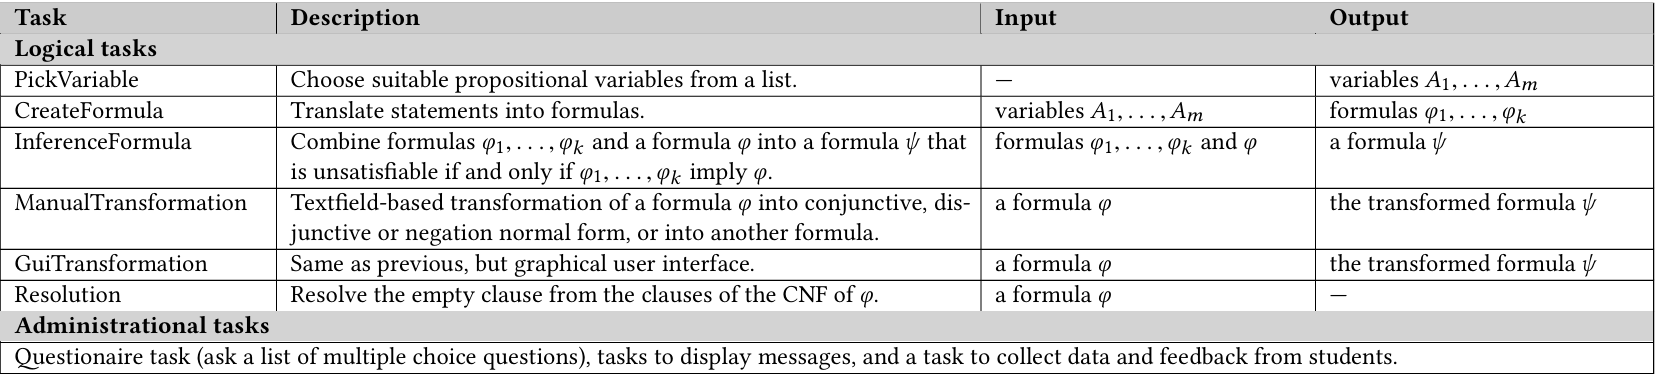
\includegraphics[width=1\linewidth]{Itils_list_of_tasks}
    \caption{List of tasks available in Iltis.}
    \label{img:iltis_tasks}
\end{figure}

From the teacher’s perspective, this framework provides a way to create more tasks. Teachers can achieve this by creating an XML file where they specify a set of tasks and a list of feedback generators to be presented to the learner.

\subsection{Feedback}
\label{chap:iltis-feedback}
Feedback generators comprise the Iltis feedback system. Teachers are allowed to associate more than one feedback generator with the task, creating different levels of assistance. Some exercises rely on feedback generators constructed using reversion rules, providing better and more accurate feedback. Reversion rules were built based on a previous study, where researchers collected some of the most frequent mistakes made by learners. A common example of a reversion rule in the “Propositional Formulas” exercises is to switch the order of the antecedent and consequent in implications. Whenever a learner switches two parameters, the feedback generator tries to apply reversion rules to find the correct solution. If successful, this indicates that the solution is close to the correct one, making it possible to provide more precise feedback based on the applied rule(s). Otherwise, it suggests that the solution is far from the correct one.

\subsection{Conclusion}
There are some positive aspects to consider from this system when developing our own tool, such as the intuitive way (it presents a low learning curve, and it is fundamental for these kinds of tools) that the exercises are presented to the learner, the advanced feedback system, and the simple access to the tool. It also provides a vast set of exercise types and a modular way to create them. On the other hand, teachers need to specify tasks in XML, and this requires some extra knowledge. Some types of exercises are still missing in this tool, like the deduction tree proof. Since it was developed by a German university and is not open-source, it cannot be expanded.

%%%%%%%%%%%%%%%%%%%%%%%%%%%%%%%%%%%%%%%%%%%%%%%%%%%%%%%%%%%%%%%%%%%
%% Logic4Fun
%%%%%%%%%%%%%%%%%%%%%%%%%%%%%%%%%%%%%%%%%%%%%%%%%%%%%%%%%%%%%%%%%%%
\section{Logic4Fun}

Logic4Fun is an online tool with a wide range of logical problems and puzzles focused on logical modeling and formalization (~\cite{slaney_logic}).

This tool has been under development since 2001 by an Australian university. It was projected to help students practice and develop skills in formalizing logical problems, as this is a challenging topic to teach, and learners often struggle with it.

Logic4Fun uses many-sorted first-order logic (MSFO) \footnote{Many-sorted first-order logic is an extension of \gls{FOL}. In \gls{FOL}, all variables come from the same domain, limiting flexibility when modeling exercises with multiple distinct domains. MSFO extends this by allowing the assignment of types (or sorts) to variables and predicates, making the language more expressive.} language to express the problems. It has a solver that takes as input a set of formulas and searches for finite models of this set. This tool presents a web page with different levels of problems: Beginner, Intermediate, Advanced, Expert, and Logician, with increasing complexity. It starts with trivial exercises to help students better understand how to use the site (declare vocabulary, set constraints, and read the solver output) and progresses to more complex and challenging exercises that require a strong background in logic. One of the key advantages of using this tool is the ability to receive immediate and accurate feedback, in contrast with traditional teaching methods. This helps keep learners motivated and encourages them to invest more time and effort into solving problems. This site also allows users to enroll in a course by using the credentials provided by the teacher.

\subsection{Feedback}

Logic4Fun tracks two kinds of errors: syntactic and semantic. Syntactic errors are mistakes in the structure or arrangement of words that violate the grammar rules of the language. These errors can be captured by the parser or type checker. When a user attempts to submit an exercise with syntactic errors, a message is presented with some suggestions. When the type checker detects an error, it provides more information, especially about the expected and given types. Semantic errors are mistakes in logic or meaning in a programming language that occur in program execution. Since there are no predefined solutions, these errors are harder to classify and to deal with. Given these difficulties, Logic4fun created a diagnostic tool to provide more informative responses to the users when a solution cannot be found. The diagnostic tool uses two approaches to provide information: approximate models and unsatisfiable cores.

\begin{itemize}
    \item In the approximate models approach, the solver starts by marking some unsatisfied constraints as "soft" and then attempts to satisfy as many as possible. Then a user can adjust constraints and rerun the solver, iterating to find the optimal approximations.
    \item In the unsatisfiable cores approach, the solver can try to identify groups of unsatisfied constraints that are causing the problem. Each group must contain at least one contradiction, giving useful clues for troubleshooting the problem.
\end{itemize}

\subsection{Conclusion}

Logic4Fun has several positive aspects, such as allowing exercises to be saved, enabling learners to pause their work and resume it later, progressively increasing the difficulty of exercises, helping learners integrate with the tool, and incorporating a diagnostic tool to address the lack of feedback. It has a class system where professors can invite their students to enroll. However, it only provides a restricted range of exercises based on first-order logic. It has some limitations with the solver's performance (the number of models presented to the user is restricted), and it is still facing issues with feedback. Sometimes, the reported errors are overly detailed or unclear, which can become frustrating for the learners.

%%%%%%%%%%%%%%%%%%%%%%%%%%%%%%%%%%%%%%%%%%%%%%%%%%%%%%%%%%%%%%%%%%%
%% LOGAX
%%%%%%%%%%%%%%%%%%%%%%%%%%%%%%%%%%%%%%%%%%%%%%%%%%%%%%%%%%%%%%%%%%%
\section{LOGAX}

LOGAX is a tool designed to help students in constructing Hilbert-style axiomatic proofs\footnote{Axiomatic proofs are a kind of proof in formal deduction where each step of the proof is supported by axioms or inference rules previously established.}. in \gls{PL} (~\cite{lodder_2020_generation}). This tool is capable of providing feedback and hints at different levels of the proofs. It can give the solutions for the steps to follow, as well as the complete solution to the problem.

The team behind LOGAX focused on various methods to provide better assistance to users during the exercises. One of the methods that they found entails the teacher providing a hidden solution or deriving it from a set of student solutions. However, this method has some drawbacks: it can only recognize solutions that are nearly identical to the stored proofs, it is limited to a fixed set of exercises, and every time a teacher wants to add a new exercise, they must provide a hidden solution. Another method that they found relies on Bolotov's algorithm, which addresses all the issues of the previous method.

Bolotov's algorithm is a proof searching algorithm for the natural deduction in \gls{FOL}.
For any given problem, if solvable, the algorithm terminates, either finding a corresponding natural deduction proof or giving a set of constraints, from which a counter-example can be extracted (~\cite{bolotov_2005_automated}).

In natural deduction, students are not strictly required to solve the exercises in one way. Proofs to the same problem can have different shapes, use different rules/axioms, and the order of the steps that the users follow can be different (\ref{chap:prop-decution}). LOGAX tool has a powerful adaptation of this algorithm that covers all the drawbacks previously mentioned in the hidden solution approach, as well as the flexible characteristics of solving Natural Deduction proofs. 

LOGAX's algorithm can adapt its solution space to better assist learners based on the user's steps. If the user takes a step in the current solution space, the algorithm can give feedback and hints directly. However, if the step diverges from the solution space, it is necessary to recalculate it, and then the system uses the new solution space to compute feedback and hints. This dynamic behavior enables the system to consistently provide feedback and hints to the user, preventing them from becoming lost in the exercise. To make this happen, the algorithm creates a directed acyclic multigraph (\gls{DAM}) that can hold more than one possible answer to a given proof. A better description of the algorithm and its adaptations can be seen in ~\cite{lodder_2020_generation, bolotov_2005_automated}. In this \gls{DAM}, vertices represent statements, and edges connect dependent statements (rule application).

Image \ref{img:dam} shows an example of generating a \gls{DAM}, where three assumptions are given (\(p\), \(p \to q\) and \(q \to r\)) and the goal is to prove \( q \to r \vdash (p \to q) \to (p \to r) \). There are solid red edges that show how to use Modus Ponens (which is the same thing as the Implication Elimination rule) and dashed blue edges that show how to use the Deduction Theorem (which is the same thing as the Implication Introduction rule). The statements \((q \to r) \to (p \to (q \to r)) \) and \( p \to (q \to r) \to ((p \to q) \to (p \to r)) \) are axioms. In this example the \gls{DAM} captures three different solutions for the same proof: one that uses axioms \(a\) and \(b\), one that uses the Deduction Theorem and axiom \(a\) and one that uses no axioms and applies the Deduction Theorem twice.

Storing this information in a \gls{DAM} makes it easier to provide feedback about the steps required to complete the proof at any given level. The user can apply the rules in any order they choose. The system can adapt to the user's solution if it diverges, simply by following the sequence of rules chosen by the user. This allows the system to easily provide information about next steps (top-down proof) or previous steps (bottom-up proof) using the edges. To provide a complete solution to the user, it is necessary to extract and trim the solutions from the \gls{DAM}.

\begin{figure}[htbp]
    \centering
    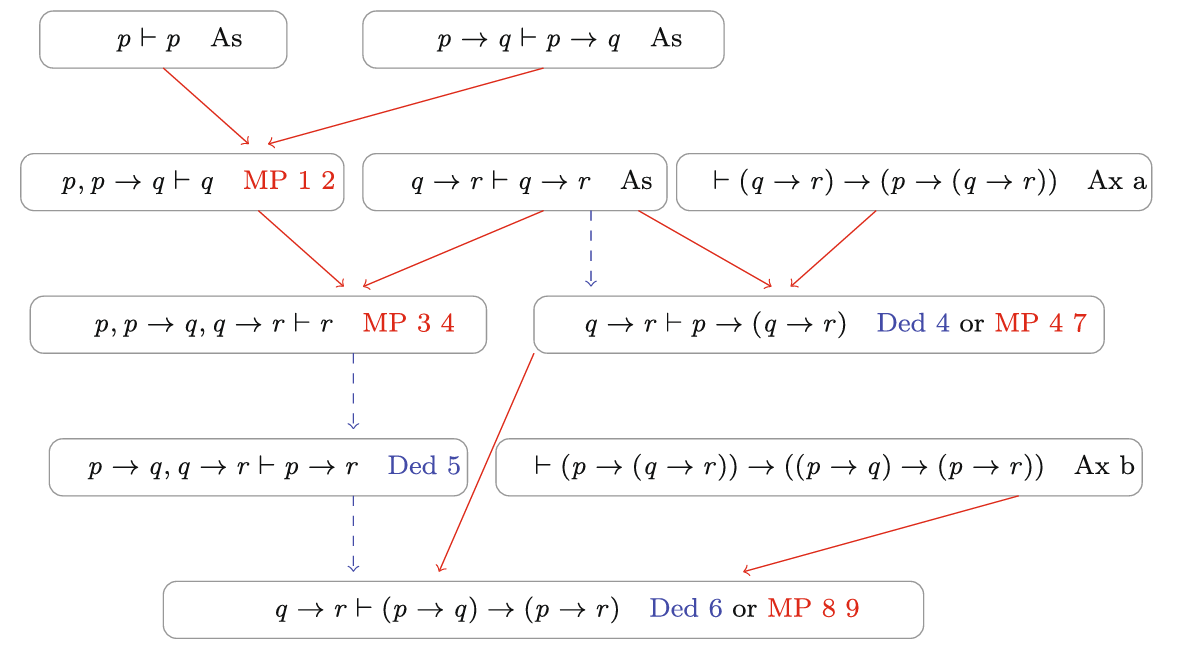
\includegraphics[width=1\linewidth]{LOGAX_DAM}
    \caption{Example of a \gls{DAM} generated by LOGAX.}
    \label{img:dam}
\end{figure}

LOGAX's team not only focused on the feedback but also the way they presented the exercises to the users. The design of this tool focuses on interfaces that allow students to concentrate on the goal of solving proofs rather than waste time figuring out syntactic errors. Shortening the number of steps and distractions required to reach the goal leads to better learning outcomes.

\subsection{Hints \& Feedback}

The LOGAX algorithm primarily covers the feedback and hints system. It can provide the directions for the next steps, indicate the next rule to be applied, and offer an explicit step-by-step procedure for performing the next step. To make the assistance system even more powerful, the team extended it to provide not only informative support but also information about subgoals. For example, rather than trying to directly prove the conclusion, the helping system offers hints in the form of sub-proofs that lead step-by-step to the final proof. By providing feedback that includes information about subgoals, the system can help students understand why a certain step is useful, and students are more likely to succeed in correcting mistakes.

The team also did some studies on students' common mistakes during proofs, and they came up with the following types of mistakes:

\begin{itemize}
    \item Oversights: Correspond to syntactic errors, for example, when a user forgets to close a parenthesis in a sentence or when logical symbols are not placed in the correct position.
    \item Conceptual errors: These occur when a student fundamentally misunderstands a concept or its application. For example, this error can occur when choosing the statements to apply a certain rule.
    \item Creative rule adaptations: These occur when students try to invent their own rules. For example, from this \( \neg p \to (q \to \neg r) \) and \( q \), we can conclude \( \neg p \to \neg r \) using Modus Ponens (Implication Elimination rule). This usually happens when the student does not know how to proceed.
\end{itemize}

The helping system underwent a final adaptation to track these mistakes. This way, the system can point out a mistake and, if possible, mention exactly which formula, subformula, or set of formulas does not match the chosen rule.

\subsection{Conclusion}

For the deduction tree exercises (REF deduc tree exercises), LOGAX appears to be a perfect fit. It covers a wide range of aspects to consider when developing a system like this. Starting with the algorithm that finds multiple possible solutions for a given proof, the fact that it ignores the order of the steps, and the ability to adjust the guidance based on the user's solution. It also includes different approaches for giving feedback and hints, as well as the idea of giving subgoals as hints to help the student understand the proof. Additionally, there are some important aspects regarding the design of the interfaces.

Unfortunately, this is an old project, and the tool is no longer available. This project has some minor drawbacks that we can consider when developing our solution. One of them is that the system doesn't provide fading strategies to reduce the amount of feedback. We might want to control the amount of feedback sent to the student based on their level of expertise. Another problem this tool faces is that the user can't erase lines of the proof. As a consequence, the final proof can be more extensive than expected. Overall, it seems to meet all the requirements for a good tutoring system, and for sure, this tool will be used as a reference for the one that we are going to develop.

%%%%%%%%%%%%%%%%%%%%%%%%%%%%%%%%%%%%%%%%%%%%%%%%%%%%%%%%%%%%%%%%%%%
%% MineFOL
%%%%%%%%%%%%%%%%%%%%%%%%%%%%%%%%%%%%%%%%%%%%%%%%%%%%%%%%%%%%%%%%%%%
\section{MineFOL}

MineFOL is a game for learning First Order Logic (~\cite{groza_minefol}). This game is very similar to a well-known game called Minesweeper. Minesweeper is a game that features a grid containing empty cells and cells with hidden mines. The object is to locate all the hidden mines using hints provided as the player explores the grid. These hints indicate the number of mines adjacent to a given cell, helping the player deduce their locations. 
MineFOL is an adaptation of that game where, instead of giving hints with the number of the nearest mines, it gives messages with \gls{FOL} expressions to help locate them, for example: \(\neg \exists x \, \text{mine}(1, x)\). These expressions are hidden in safe squares, and the goal is to find the maximum number of expressions to have enough information to locate all mines in as few steps as possible. The player can only travel through safe squares. A square is considered safe if it is possible to prove it using the collected messages. If the player steps out of the proven zone, the game ends. The game always starts at the top left corner of the grid(\(cell(1,1)\)) with an initial expression. Players always have information about how many mines there are and the maximum number of moves to solve the problem. We can combine this information with the collected expressions to extract more valuable insights. Image \ref{img:minefol} illustrates a game where the objective is to locate one mine within 35 movements.

\begin{figure}[htbp]
    \centering
    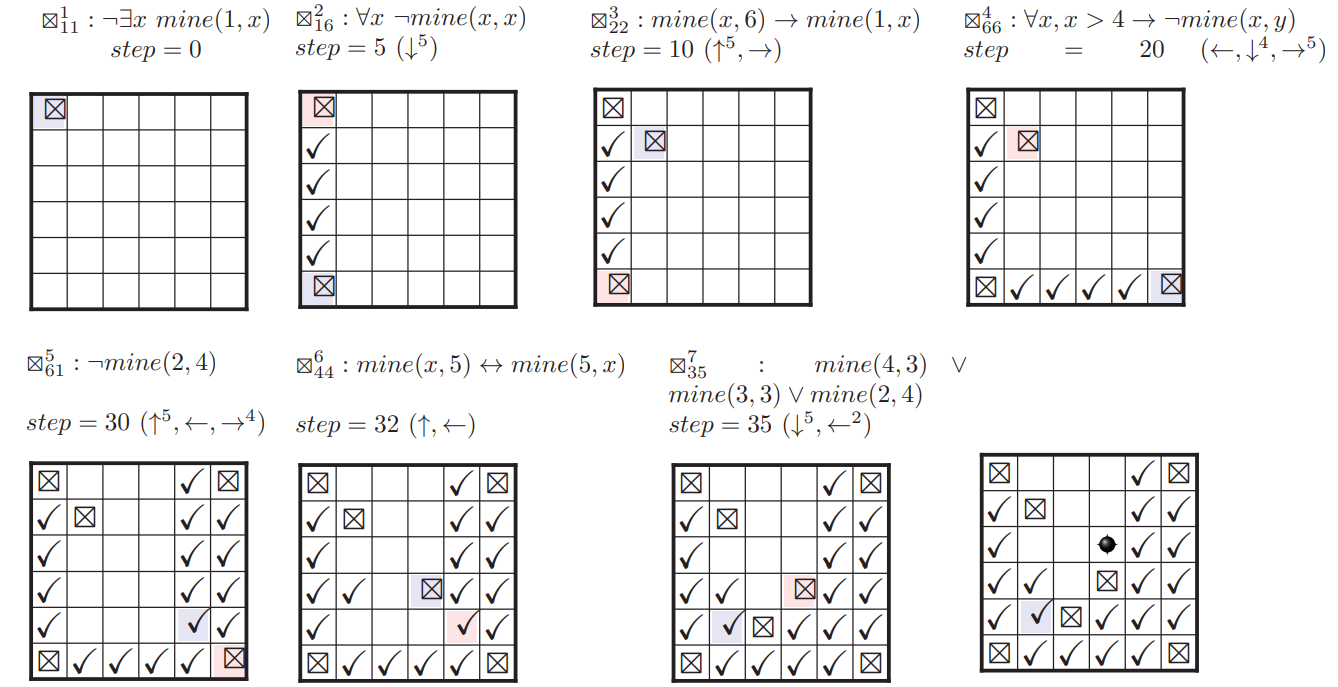
\includegraphics[width=1\linewidth]{MineFOL}
    \caption{MineFOL example with one mine and 35 movements. Blue squares represent the player's current position, and the red ones represent the previous position. Cells with: \(\boxtimes\) contain a message and \( \checkmark \) represent safe squares.}
    \label{img:minefol}
\end{figure}

MineFOL has three different modes:

\begin{itemize}
    \item "Play it yourself!": In this mode the user tries to locate all mines based on a set of discovered \gls{FOL} expressions. This can help the student practice reasoning in \gls{FOL}, since the student has to translate the expressions to natural language to understand the message in order to solve the game.
    \item "Challenge a software agent!": In this mode, the computer is responsible for solving the game. The student doesn't need to worry about anything. If the game is valid, the agent will find a solution for it, and they will present it to the student.
    \item "Create your own game!": In this mode, the user is responsible for setting up the game. Students can define their own \gls{FOL} expressions, as well as the size of the grid and the number of mines. The complexity of the game can vary based on the grid size, the number of mines, the size and complexity of the \gls{FOL} expressions, and the number of steps required to complete it. This mode is a good way for students to practice formalization in \gls{FOL}. To check if the game is valid (can be solved), the student can challenge the software agent.
\end{itemize}

\subsection{Feedback}
This game includes a feedback system that provides assistance every time the player loses a game. When a player leaves the safe zone, the system provides an explanation of why the cell is unsafe by displaying a resolution-based proof.

\subsection{Conclusion}
MineFOL introduces a new concept that none of the previously described tools has. The concept of gamification consists of applying game mechanics and concepts in non-gaming environments. Studies show that if the learning platform is gamified, it does not only drastically increase the user enrollment but also increase user engagement throughout the course (~\cite{vaibhav_gamification}). Using MineFOL, students develop skills in reasoning and formalization while playing the game. It also allows competitiveness and creativity between students by creating and challenging other students to complete their own maps. The game also has different levels of complexity, allowing students with less experience to have a chance to learn, while more advanced students can challenge themselves with harder levels to further improve their skills.


%\section{Iltis}
%\subsection{Conclusion}